
%
% File abstract.tex


\documentclass[11pt,a4paper,table]{article}
\usepackage{authblk}
\usepackage[hyperref]{acl2019}
\usepackage{times}
\usepackage{latexsym}
\usepackage{url}
\usepackage{xr}
\usepackage[T1]{fontenc}
\usepackage[scaled=.8]{beramono}
\usepackage[scaled=.95]{helvet}
\usepackage{amsmath}
\usepackage{color,soul}
\usepackage{subcaption}
\usepackage[font=10pt,labelfont=bf,skip=5pt]{caption}
\usepackage[shortlabels]{enumitem} % customizable lists
\usepackage{multirow}
\usepackage{tikz}
\usepackage{tikz-dependency}
\usepackage[warn]{textcomp}
\usepackage{etoolbox}
\usepackage{xfrac}
\usepackage{pgfplotstable}
\usepackage{tabularx}
\usepackage{collcell}
\usepackage{booktabs}
\usepackage{nameref}
\usepackage{cleveref}

\aclfinalcopy % Uncomment this line for the final submission

%\setlength\titlebox{5cm}
% You can expand the titlebox if you need extra space
% to show all the authors. Please do not make the titlebox
% smaller than 5cm (the original size); we will check this
% in the camera-ready version and ask you to change it back.

\pgfplotsset{compat=1.15}
\makeatletter
\newcommand*{\addFileDependency}[1]{% argument=file name and extension
  \typeout{(#1)}
  \@addtofilelist{#1}
  \IfFileExists{#1}{}{\typeout{No file #1.}}
}
\makeatother
 
\newcommand*{\myexternaldocument}[1]{%
    \externaldocument{#1}%
    \addFileDependency{#1.tex}%
    \addFileDependency{#1.aux}%
}

% use \S for all references to all kinds of sections, and \P to paragraphs
% (sadly, we cannot use the simpler \crefname{} macro because it would insert a space after the symbol)
\crefformat{part}{\S#2#1#3}
\crefformat{chapter}{\S#2#1#3}
\crefformat{section}{\S#2#1#3}
\crefformat{subsection}{\S#2#1#3}
\crefformat{subsubsection}{\S#2#1#3}
\crefformat{paragraph}{\P#2#1#3}
\crefformat{subparagraph}{\P#2#1#3}
%\crefmultiformat{part}{\S#2#1#3}{ and~\S#2#1#3}{, \S#2#1#3}{, and~\S#2#1#3}
%\crefmultiformat{chapter}{\S#2#1#3}{ and~\S#2#1#3}{, \S#2#1#3}{, and~\S#2#1#3}
\crefmultiformat{section}{\S#2#1#3}{ and~\S#2#1#3}{, \S#2#1#3}{, and~\S#2#1#3}
\crefmultiformat{subsection}{\S#2#1#3}{ and~\S#2#1#3}{, \S#2#1#3}{, and~\S#2#1#3}
\crefmultiformat{subsubsection}{\S#2#1#3}{ and~\S#2#1#3}{, \S#2#1#3}{, and~\S#2#1#3}
\crefmultiformat{paragraph}{\P\P#2#1#3}{ and~#2#1#3}{, #2#1#3}{, and~#2#1#3}
\crefmultiformat{subparagraph}{\P\P#2#1#3}{ and~#2#1#3}{, #2#1#3}{, and~#2#1#3}
%\crefrangeformat{part}{\mbox{\S\S#3#1#4--#5#2#6}}
%\crefrangeformat{chapter}{\mbox{\S\S#3#1#4--#5#2#6}}
\crefrangeformat{section}{\mbox{\S\S#3#1#4--#5#2#6}}
\crefrangeformat{subsection}{\mbox{\S\S#3#1#4--#5#2#6}}
\crefrangeformat{subsubsection}{\mbox{\S\S#3#1#4--#5#2#6}}
\crefrangeformat{paragraph}{\mbox{\P\P#3#1#4--#5#2#6}}
\crefrangeformat{subparagraph}{\mbox{\P\P#3#1#4--#5#2#6}}
% for \label[appsec]{...}
\crefname{part}{Part}{Parts}
\Crefname{part}{Part}{Parts}
\crefname{chapter}{ch.}{ch.}
\Crefname{chapter}{Ch.}{Ch.}
\crefname{figure}{figure}{figures}
\crefname{subfigure}{figure}{figures}
\Crefname{subfigure}{Figure}{Figures}
\crefname{appsec}{appendix}{appendices}
\Crefname{appsec}{Appendix}{Appendices}
\crefname{algocf}{algorithm}{algorithms}
\Crefname{algocf}{Algorithm}{Algorithms}
\crefname{enums,enumsi}{example}{examples}
\Crefname{enums,enumsi}{Example}{Examples}
\crefname{}{example}{examples} % lingmacros \toplabel has no internal name for the kind of label
\Crefname{}{Example}{Examples}
\crefformat{enums}{(#2#1#3)}
\crefformat{enumsi}{(#2#1#3)}
\crefrangeformat{enums}{\mbox{(#3#1#4--#5#2#6)}}
\crefrangeformat{enumsi}{\mbox{(#3#1#4--#5#2#6)}}
\crefformat{}{(#2#1#3)}
\crefname{xnumi}{example}{examples} % gb4e
\crefname{xnumi}{example}{examples} % gb4e
\Crefname{xnumii}{Example}{Examples} % gb4e
\Crefname{xnumii}{Example}{Examples} % gb4e
\crefformat{xnumi}{(#2#1#3)} % gb4e
\crefformat{xnumii}{(#2#1#3)} % gb4e
\crefrangeformat{enums}{\mbox{(#3#1#4--#5#2#6)}}
\crefrangeformat{enumsi}{\mbox{(#3#1#4--#5#2#6)}}
\crefrangeformat{xnumi}{\mbox{(#3#1#4--#5#2#6)}} % gb4e
\crefrangeformat{xnumii}{\mbox{(#3#1#4--#5#2#6)}} % gb4e
\crefmultiformat{enumsi}{(#2#1#3}{, #2#1#3)}{, #2#1#3}{, #2#1#3)}
\crefmultiformat{xnumi}{(#2#1#3}{, #2#1#3)}{, #2#1#3}{, #2#1#3)} % gb4e
\crefmultiformat{xnumii}{(#2#1#3}{, #2#1#3)}{, #2#1#3}{, #2#1#3)} % gb4e
\crefrangemultiformat{enumsi}{(#3#1#4--#5#2#6}{, #3#1#4--#5#2#6)}{, #3#1#4--#5#2#6}{, #3#1#4--#5#2#6)}
\crefrangemultiformat{xnumi}{(#3#1#4--#5#2#6}{, #3#1#4--#5#2#6)}{, #3#1#4--#5#2#6}{, #3#1#4--#5#2#6)} % gb4e
\crefrangemultiformat{xnumii}{(#3#1#4--#5#2#6}{, #3#1#4--#5#2#6)}{, #3#1#4--#5#2#6}{, #3#1#4--#5#2#6)} % gb4e

\ifx\creflastconjunction\undefined%
\newcommand{\creflastconjunction}{, and\nobreakspace} % Oxford comma for lists
\else%
\renewcommand{\creflastconjunction}{, and\nobreakspace} % Oxford comma for lists
\fi%

\newcommand*{\Fullref}[1]{\hyperref[{#1}]{\Cref*{#1}: \nameref*{#1}}}
\newcommand*{\fullref}[1]{\hyperref[{#1}]{\cref*{#1}: \nameref{#1}}}
\newcommand{\fnref}[1]{fn.~\ref{#1}} % don't use \cref{} due to bug in (now out-of-date) cleveref package w.r.t. footnotes
\newcommand{\Fnref}[1]{Fn.~\ref{#1}}

\newcommand{\citeposs}[2][]{\citeauthor{#2}'s (\citeyear[#1]{#2})}
\newcommand{\Citeposs}[2][]{\Citeauthor{#2}'s (\citeyear[#1]{#2})}



% \makeatletter
% \renewcommand{\@BIBLABEL}{\@emptybiblabel}
% \newcommand{\@emptybiblabel}[1]{}
% \makeatother
\DeclareMathOperator*{\argmax}{arg\,max}

\newcommand{\ucca}[1]{\textcolor{gray}{\textbf{\textsf{#1}}}}
\newcommand{\sst}[1]{\textsc{#1}}
\newcommand{\lexcat}[1]{\textsl{#1}}


\definecolor{orange}{rgb}{1,0.5,0}
\definecolor{mdgreen}{rgb}{0.05,0.6,0.05}
\definecolor{Acolor}{HTML}{EC5D57} % poppy red
\definecolor{Pcolor}{HTML}{70BF41} % grass green
\definecolor{Scolor}{HTML}{51A7F9} % sky blue
\definecolor{Lcolor}{HTML}{B36AE2} % friendly purple
\definecolor{mdblue}{rgb}{0,0,0.7}
\definecolor{dkblue}{rgb}{0,0,0.5}
\definecolor{dkgray}{rgb}{0.3,0.3,0.3}
\definecolor{slate}{rgb}{0.25,0.25,0.4}
\definecolor{gray}{rgb}{0.5,0.5,0.5}
\definecolor{ltgray}{rgb}{0.7,0.7,0.7}
\definecolor{purple}{rgb}{0.7,0,1.0}
\definecolor{lavender}{rgb}{0.65,0.55,1.0}



\newcommand{\com}[1]{}
\newcommand{\oa}[1]{\textcolor{red}{[OA: #1]}}
\newcommand{\daniel}[1]{\footnote{\color{cyan}DH: #1}}
\newcommand{\nss}[1]{\textcolor{magenta}{[NSS: #1]}}

\newcommand{\finalversion}[1]{} % hide for now, restore for camera-ready

\hyphenation{English}
\hyphenation{PredPatt}
\hyphenation{WordNet}
\hyphenation{WordNets}
\hyphenation{FrameNet}
\hyphenation{SemCor}
\hyphenation{SemEval}
\hyphenation{ParsedSemCor}
\hyphenation{VerbNet}
\hyphenation{PennConverter}
\hyphenation{an-aly-sis}
\hyphenation{an-aly-ses}
\hyphenation{base-line}
\hyphenation{comb-over}
\hyphenation{de-ve-lop-ed}
\hyphenation{news-text}
\hyphenation{nomi-nal}
\hyphenation{per-cept}
\hyphenation{per-cepts}
\hyphenation{post-edit-ing}
\hyphenation{shriv-eled}
\hyphenation{Huddle-ston}
\hyphenation{par-ti-ci-pant}
\hyphenation{par-ti-ci-pants}
\hyphenation{par-ti-ci-pa-tion}

%\setlength{\belowcaptionskip}{-10pt}
%\setlength{\parskip}{-0.085mm}

%\lstset{basicstyle=\ttfamily}


\usetikzlibrary{shapes,shapes.misc}

% for confusion matrix
\newcommand{\ApplyGradient}[1]{%
  \pgfmathsetmacro{\PercentColor}{(#1-0)/7.97}%
  \pgfmathsetmacro{\PercentInverse}{ifthenelse(\PercentColor > 65, 0, 100)}%
  %\textcolor{black!\PercentColor}{#1}
  \edef\x{\noexpand\cellcolor{red!\PercentColor}}\x\textcolor{black!\PercentInverse}{#1}%
}
\newcolumntype{R}{>{\small\collectcell\ApplyGradient}{c}<{\endcollectcell}}

%\def\arraystretch{1.1}
\renewcommand{\labelenumii}{\theenumii}
\renewcommand{\theenumii}{\theenumi.\arabic{enumii}.}

\title{Tutorial at COLING 2020 \\
Cross-lingual Semantic Representation for NLP with UCCA \\
\normalsize\url{https://github.com/UniversalConceptualCognitiveAnnotation/tutorial}}

\author[*]{\textbf{Omri Abend}}
\author[*]{\textbf{Dotan Dvir}}
\author[**]{\textbf{Daniel Hershcovich}}
\author[***]{\textbf{Jakob Prange}}
\author[***]{\textbf{Nathan Schneider}}
\affil[*]{Hebrew University of Jerusalem}
\affil[**]{University of Copenhagen}
\affil[***]{Georgetown University}
\affil[ ]{
\texttt{oabend@cs.huji.ac.il},\quad
\texttt{dotan.dvir@mail.huji.ac.il},\quad
\texttt{dh@di.ku.dk}}
\affil[ ]{
\texttt{jakob@cs.georgetown.edu},\quad
\texttt{nathan.schneider@georgetown.edu}
}

\begin{document}

\maketitle

\begin{abstract}
This is an introductory tutorial to UCCA (Universal Conceptual Cognitive Annotation), a cross-linguistically applicable framework for semantic representation, with corpora annotated in English, German and French, and ongoing annotation in Russian and Hebrew. UCCA builds on extensive typological work and supports rapid annotation. The tutorial will provide a detailed introduction to the UCCA annotation guidelines, design philosophy and the available resources; and a comparison to other meaning representations. It will also survey the existing parsing work, including the findings of two recent shared tasks, in SemEval and CoNLL, that addressed UCCA parsing. Finally, the tutorial will present recent applications and extensions to the scheme, demonstrating its value for natural language processing in a range of languages and domains.
\end{abstract}


\section{Introduction}\label{sec:introduction}

Universal Conceptual Cognitive Annotation \cite[UCCA;][]{abend2013universal} 
is a symbolic meaning representation (MR)
that supports human annotation of text with broad coverage.
While several meaning representation schemes share this goal
\citep{abend2017state}, UCCA targets a level of semantic granularity that abstracts away from syntactic paraphrases in a typologically-motivated, cross-linguistic fashion, building on Basic Linguistic Theory \citep{Dixon:basic}, an influential framework for linguistic description.
The scheme does not rely on language-specific resources, and sets a low
threshold for annotator training.

UCCA has been annotated on several corpora of different genres and
languages,\footnote{\scriptsize\url{https://github.com/UniversalConceptualCognitiveAnnotation}} as summarized in \cref{tab:data}.
Pilot studies have been conducted in additional languages.
A web-based annotation system is available \cite{abend2017uccaapp}.

In UCCA, an analysis of a text passage is a directed acyclic graph
over semantic elements called \textit{units}.
The principal kind of unit is a \textit{scene},
which describes an action, movement or state, and is similar to FrameNet's notion of a {\it frame}.
\Cref{fig:ex} contains three scenes, evoked, respectively,
by the verb \textit{took},
the noun phrase \textit{a repair}, and the possessive \textit{our}.
Several elements are exemplified, including participants,
secondary relations, and scene linkage.
The graph is anchored in the text tokens (the leaves generally correspond to one or more tokens), and relations between units
are indicated by the \textit{categories} assigned to the edges connecting them.

The goals of this tutorial are:
to describe the UCCA representation as a linguistic scheme and how it is
being used computationally, especially for cross-lingual and multilingual
NLP; to familiarize participants with existing UCCA parsers and
equip them with the conceptual tools required for desigining new parsers;
and to review existing extensions and possible future directions.

\begin{table}[t]
\centering\setlength{\tabcolsep}{3.5pt}
\begin{tabular}{ll|rr}
& \bf Genre & \bf \# Tokens & \bf \# Sentences \\
\hline
\multicolumn{2}{l|}{\bf English} \\
Wiki & Encyclopedia & 158,573 & 5,141 \\
20k & Literary & 12,574 & 492 \\
EWT & Online reviews & 55,590 & 3,813 \\
WSJ & Financial news & 2,273 & 100 \\
LPP & Literary & 1,322 & 100 \\\hline
\multicolumn{2}{l|}{\bf German} \\
20k & Literary & 144,531 & 6,510 \\
LPP & Literary & 18,653 & 1,042 \\\hline
\multicolumn{2}{l|}{\bf French} \\
20k & Literary & 12,954 & 492 \\\hline
\multicolumn{2}{l|}{\bf Hebrew, Russian} \\
LPP & Literary & \multicolumn{2}{c}{annotation underway}\\\hline
\end{tabular}
\caption{Data statistics for existing UCCA corpora.\label{tab:data}}
\end{table}

\begin{figure*}[t]\centering
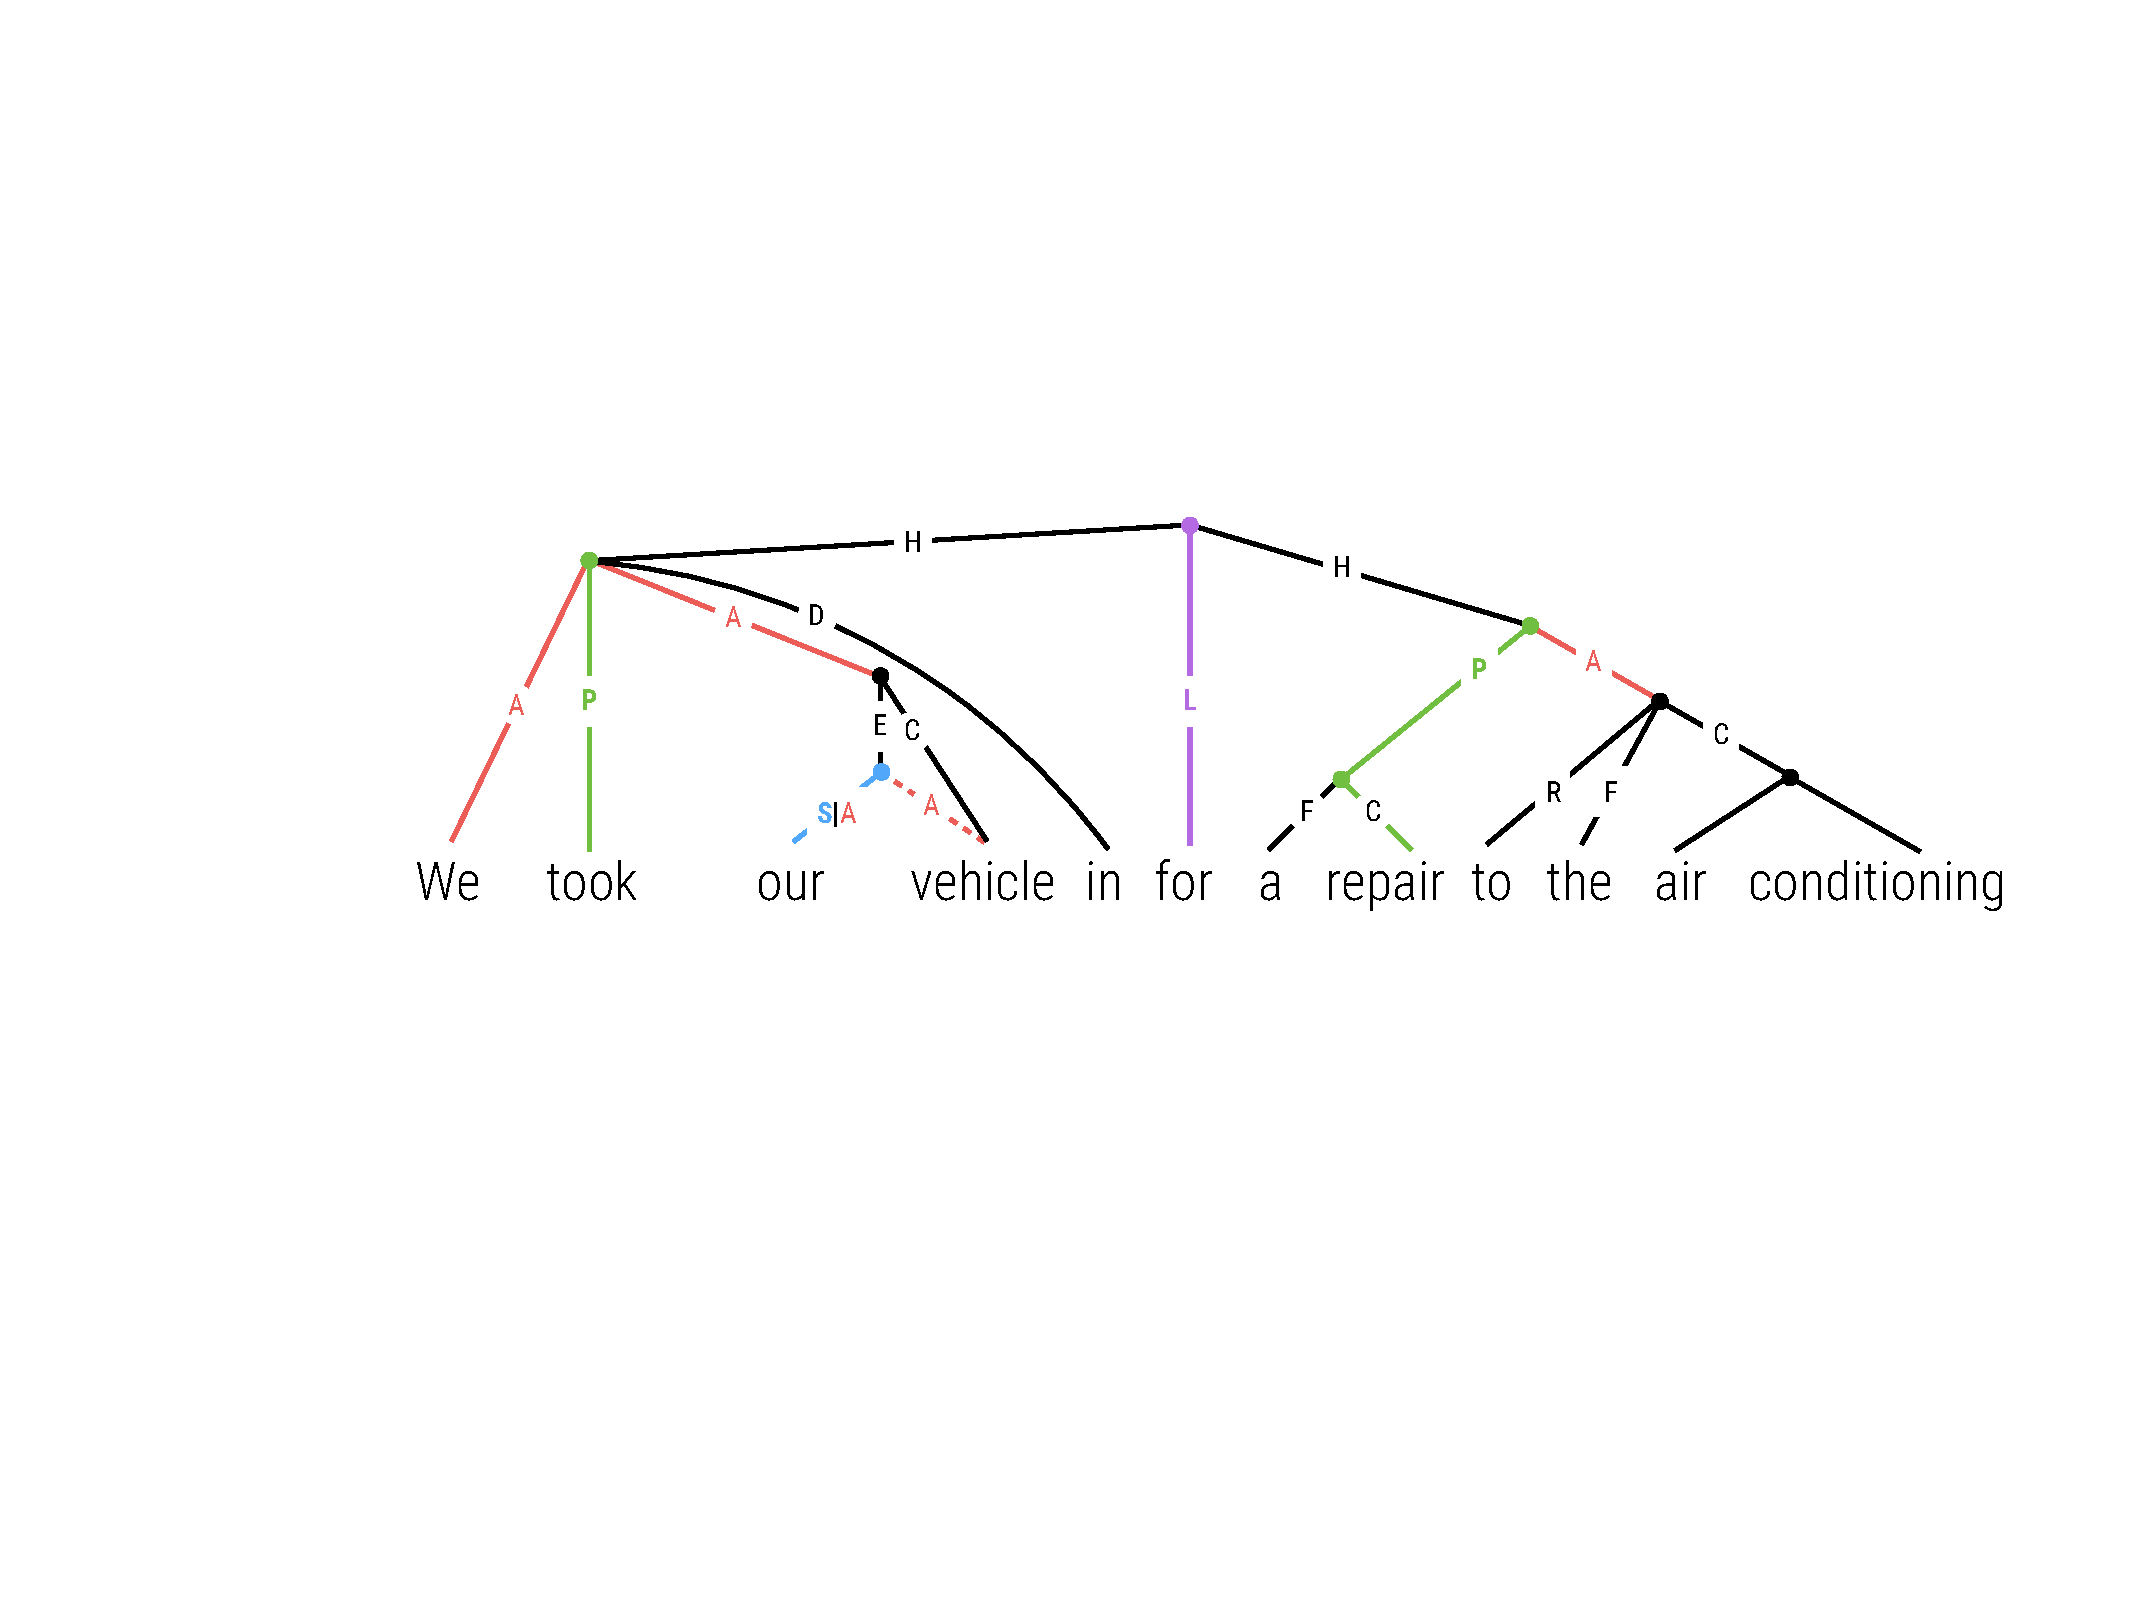
\includegraphics[width=\textwidth]{ex-ucca.pdf}
\caption{Example sentence from EWT (\texttt{reviews-086839-0003}),
with its UCCA annotation.
Category abbreviations: \ucca{\color{black}H} = parallel scene, \ucca{\color{Lcolor}L} = scene linker, \ucca{\color{Pcolor}P} = process (dynamic event), \ucca{\color{Scolor}S} = state, \ucca{\color{Acolor}A} = scene participant, \ucca{\color{black}D} = scene adverbial, \ucca{\color{black}E} = non-scene elaborator, \ucca{\color{black}C} = center (non-scene head), \ucca{\color{black}R} = relator, \ucca{\color{black}F} = functional element.}
\label{fig:ex}
\end{figure*}

%%%%%%%%%%%%%%%%%%%%%%%%%%%%%%%%%%%%%%%%%%%%%%%%%%%%%%%%%%%%%%%%%%%%%%%%%%%%

\section{Relevance}\label{sec:relevance}

UCCA resources and applications are valuable for cross-lingual NLP:
like Universal Dependencies \cite[UD;][]{11234/1-2988},
UCCA's category set can in principle be applied to a wide variety of languages.
It is also cross-linguistically stable, and reflects a level of semantic structure that is usually preserved in translations \cite{sulem2015conceptual}.
UCCA has been applied in NLP to text simplification \citep{sulem2018simple},
and text-to-text generation evaluation \citep{birch2016hume,marecek-etal-2017-cuni,choshen2018usim,sulem2018samsa,alvamanchego-etal:2019:easse}.
The tutorial will describe the guidelines and rationale behind UCCA,
helping potential application designers understand what abstractions
it makes.

Significant effort has been devoted to building UCCA parsers
\cite{hershcovich2017a,jiang-19,zhang2019broad},
including a SemEval~2019 shared task
on cross-lingual UCCA parsing \citep{hershcovich2019shared},
which had 8 participating teams,
and a CoNLL~2019 shared task on cross-framework meaning representation
parsing \cite{Oep:Abe:Haj:19},
where 12 teams submitted parsed UCCA graphs.
This tutorial will allow researchers interested in UCCA parsing, and more generally graph parsing, deepen their understanding of the framework, 
and what properties make it unique.
The tutorial will include a brief survey of the various approaches taken by existing parsers, and prepare attendees to work on UCCA parsing themselves.

Furthermore, UCCA parsing has been shown to benefit from multi-task learning
\cite{caruana1998multitask}
with other meaning representations \cite{hershcovich2018multitask}, and
preliminary results from the CoNLL 2019 shared task \cite{Oep:Abe:Haj:19}
show that it is also useful as an auxiliary task in itself.
The tutorial will compare and contrast UCCA and other meaning representations,
and will thereby inform participants of the potential advantages and difficulties
in employing multi-task learning across semantic schemes.

UCCA defines a small inventory of coarse-grained categories so as not to rely on language-specific lexical resources, and  can thus in principle be applied to a great variety of languages. This distinguishes UCCA from finer-grained sentence-structural representations like FrameNet \citep{Baker:98}, the Abstract Meaning Representation \citep[AMR;][]{banarescu2013abstract}, which relies on PropBank \citep{Palmer:05},
and Universal Decompositional Semantics \citep[Decomp;][]{white2016universal}.
For example, FrameNet requires a different ontology for each new language addressed \cite{ohara2003japanese,You2005BuildingCF,borin20132,park2014frame,hayoun-elhadad-2016-hebrew,djemaa-etal-2016-corpus},
and AMR underwent significant customization to be applicable to Chinese
\cite{li-etal-2016-annotating}. Decomp takes a different approach to multilinguality, where the parser is required to parse sentences in other languages to their corresponding {\it English} semantic forms \citep{zhang2018cross}.
The tutorial will address contemporary issues in the field, such as
the question of how to represent semantic structure multilingually with
broad coverage, which is actively being explored from many angles.

While UCCA structures and categories are intentionally coarse, the scheme has a multi-layered architecture, which allows for refinement using additional {\it layers}, which serve as ``modules'' of semantic distinctions.
We will give an overview of the recently proposed extensions
(to support coreference) and joint parsing experiments \citep{prange2019made,prange2019semantically}.

%%%%%%%%%%%%%%%%%%%%%%%%%%%%%%%%%%%%%%%%%%%%%%%%%%%%%%%%%%%%%%%%%%%%%%%%%%%%

\section{Agenda}\label{sec:agenda}

% The first half of the tutorial will provide an in-depth introduction to the annotation scheme, and the second half, being more of a literature survey, will split roughly equally between work by the tutorial presenters, and others'.\oa{what purpose does this sentence serve?}
The planned division of time is as follows:

\begin{enumerate}
    \item \textbf{Bird's eye view (45m).}
    Design philosophy, notion of scenes, basic explanation of categories, simple examples.
    \item \textbf{Annotation guidelines (35m).}
    Linguistic details, interesting constructions
    in several languages.
    \item \textbf{Data and annotation (10m).}
    Overview of annotated data (see \S\ref{sec:introduction})
    and the annotation process and software \cite{abend2017uccaapp}.
    \begin{center}
        COFFEE BREAK
    \end{center}
    \item \textbf{Extensions to UCCA and integration with other schemes (15m).}
    Semantic roles \cite{prange2019made} and
    coreference \cite{prange2019semantically}.
    \item \textbf{Relation to other representations (15m).}
    Comparison to other meaning representations
    \cite{abend2017state,koller2019graph}
    and to UD \cite{hershcovich2019content}.
    \item \textbf{Parsing (25m).}
    TUPA \cite{hershcovich2017a,hershcovich2018multitask},
    SemEval~2019 Task~1 \cite{hershcovich2019shared,jiang-19},
    CoNLL~2019 Shared Task \cite{Oep:Abe:Haj:19}, and
    more recent parsers \cite{zhang2019broad}.
    \item \textbf{Monolingual tasks and evaluation (20m).}
    Sentence simplification \cite{sulem2018simple},
    evaluation of sentence simplification \cite{sulem2018samsa,alvamanchego-etal:2019:easse}
    and grammatical error correction \cite{choshen2018usim}.
    \item \textbf{Cross-linguistic studies and applications (15m).}
    Analysis of cross-linguistic stability \cite{sulem2015conceptual},
    machine translation evaluation \cite{birch2016hume,marecek-etal-2017-cuni}.
\end{enumerate}

\subsection{Prerequisites}\label{sec:prerequisites}

No prior knowledge is assumed about linguistics and typology.
The necessary background will be provided as part of the tutorial.
However, participants are expected to know about basic data structures
such as trees and graphs.
For the parsing section, prior knowledge is assumed about
common machine learning techniques, including supervised learning
and neural networks.

\subsection{Reading list}\label{sec:reading}

The following are recommended to read before the tutorial, as
they provide background and frame the context in which the tutorial
materials lie:

\begin{enumerate}
    \item Chapter 3 of \Citet{Dixon:05} contains an introduction
    to some basic concepts in semantics on which UCCA is based.
    \item \Citet{kiperwasser-goldberg-2016-simple} present a
    transition-based parser using an architecture on which TUPA, the first
    UCCA parser, is based \cite{hershcovich2017a}.
    \item \Citet{P17-1186} performed multi-task learning for
    meaning representation parsing, inspiring work on cross-framework
    parsing for UCCA \cite{hershcovich2018multitask}.
    \item \Citet{abend2017state} compare and constrast several meaning
    representations according to various aspects.
    \item \Citet{deng2017translation} investigate translation divergences
    using a hierarchical alignment,
    and discuss bridging them with cross-lingual semantic representations.
    \item \Citet{croft2017linguistic} list typologically-informed design 
    criteria for Universal Dependencies \cite{11234/1-2988},
    which are also relevant for other structural representations in NLP.
    % \item \Citet{hershcovich2019shared} summarize the SemEval~2019 shared task on cross-lingual UCCA parsing.
    % \item \Citet{jiang-19} describe the HLT@SUDA parser, winner of the SemEval~2019 shared task based on a constituency tree parser.
    % \item \Citet{lyu-etal-2019-cuny} describe the CUNY-PKU parser, a
    % strong ensemble-based submission in the SemEval~2019 shared task.
    % \item \Citet{Oep:Abe:Haj:19} summarize the CoNLL~2019 shared task on cross-framework meaning representation parsing, targeting UCCA and four other frameworks.
    % \item \Citet{zhang2019broad} present a transduction-based
    % semantic parser that is competitive on UCCA and two other
    % meaning representations.
\end{enumerate}

\section{Presenters}\label{sec:instructors}

The instruction in this tutorial involves organizers at various
career stages, exhibiting geographic diversity, and diversity in terms of 
gender.

\textbf{Omri Abend} (\url{https://www.cse.huji.ac.il/~oabend})
is a Senior Lecturer (Assistant Professor) of Computer Science and Cognitive Science
at the Hebrew University of Jerusalem.
Research interests:
computational semantics and specifically, cross-linguistically applicable
semantic and grammatical representation, semantic parsing, corpus annotation and evaluation.
Relevant experience: co-developer of the UCCA scheme, partner in all annotation and application efforts related to UCCA, and in some of the parsing efforts. Publishes regularly in NLP conferences (ACL, NAACL, EMNLP etc.).

\textbf{Dotan Dvir} has been managing the UCCA manual annotation project at the Hebrew University of Jerusalem since 2017. She was involved in writing version 2 of the UCCA guidelines. She has in-depth knowledge of the UCCA guidelines and is experienced in instructing annotators about them. Before joining the UCCA project, she had been working as a text analyst in IBM's Project Debater (2014-2017).

\textbf{Daniel Hershcovich} (\url{https://danielhers.github.io})
is a Tenure-Track Assistant Professor at the University of Copenhagen, Denmark.
Daniel pioneered the work on UCCA parsing, and
is interested in semantic parsing and meaning representations.
Daniel develops and maintains the UCCA toolkit Python codebase,\footnote{\url{https://github.com/danielhers/ucca}}
has teaching experience in an NLP course
at the Hebrew University of Jerusalem,
and publishes in NLP conferences.

\textbf{Jakob Prange} (\url{https://prange.jakob.georgetown.domains})
is pursuing his Ph.D. at Georgetown University, investigating design, annotation, and parsing strategies for various meaning representations.
Among other formalisms (SNACS, frame semantics, STAG, CCG), he has studied and worked with UCCA over the past two years, which recently resulted in two published proposals of novel UCCA extensions, for coreference and semantic roles.
He has experience with teaching in multicultural classroom settings and presenting research at international conferences.

\textbf{Nathan Schneider} (\url{http://nathan.cl})
leads an interdisciplinary computational linguistics research group at Georgetown University. 
He has worked on the design and parsing of a range of broad-coverage representations for different aspects and granularities of meaning, including multiword expressions, supersenses, frame semantics, AMR, and UCCA (as a multiyear collaboration with the copresenters). 
He has experience teaching meaning representations in classroom settings as well as conference tutorials---notably, a tutorial on AMR \citep{amrtutorial} whose materials\footnote{\url{https://github.com/nschneid/amr-tutorial/}} continue to serve as a useful introduction to the scheme, 
and will serve as a model for the proposed UCCA tutorial.

\bibliography{references}
\bibliographystyle{acl_natbib}

\end{document}
